%Correctness
\section{Correctness}
\subsection{The Graph Structure}
\begin{figure}[htb]
    \centering
    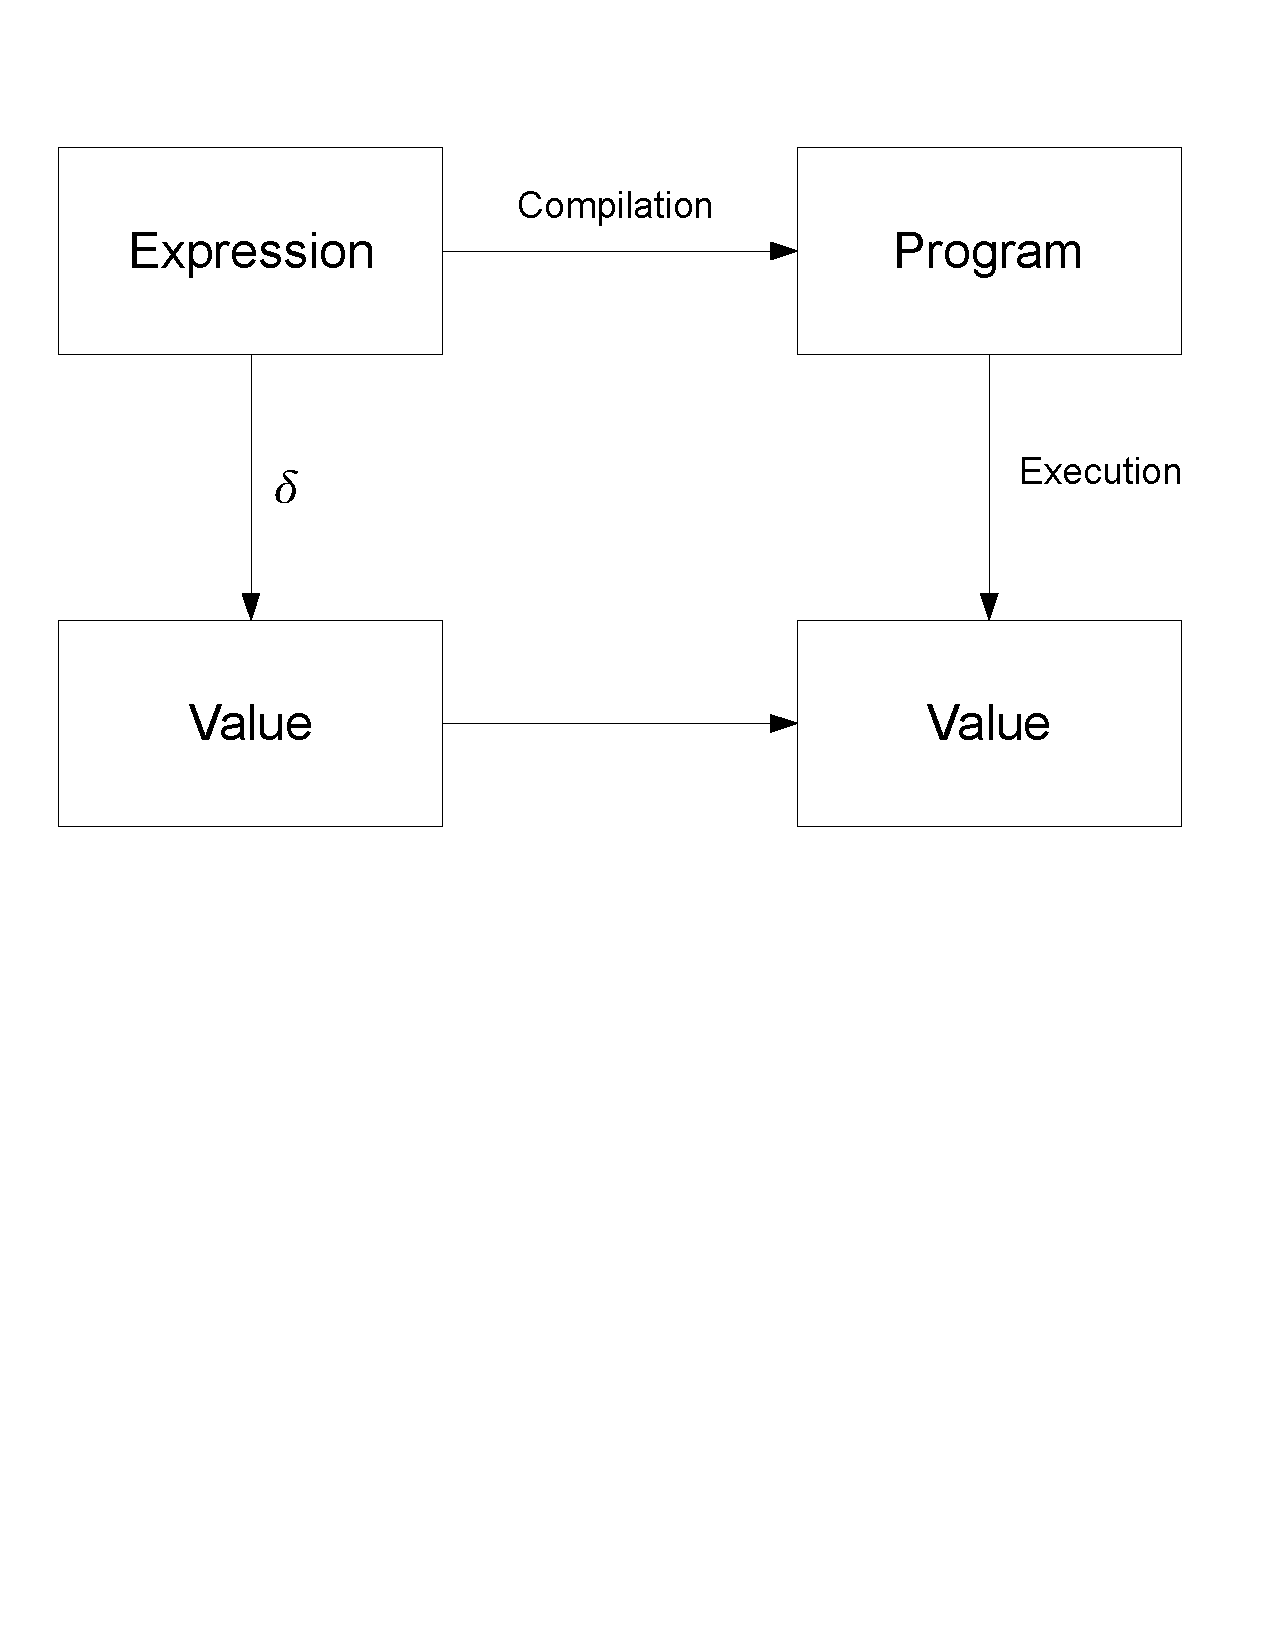
\includegraphics[trim= 10mm 120mm 10mm 10mm, clip, width=250px]{./images/correctness_graph1.pdf}
    \caption{Code Transformations}
    \label{fig:correctness_graph1}
\end{figure}
The graph structure chosen is simple directed graph in which the syntax and semantics are discussed in detail in sections \ref{sec:statechartsyn}, \ref{sec:statechartsem} respectively. Our program peforms transformations on the diagram to form code constructs. In order to show correctness we will demonstrate that our transformations follow figure \ref{fig:correctness_graph1}. Figure \ref{fig:correctness_graph1} essentially says that a simulated evaluation of each expression ($\delta$) to a value will be equivalent to the actual executed program of the same value. In addition we also need to prove the program structure
\begin{figure}[htb]
    \centering
    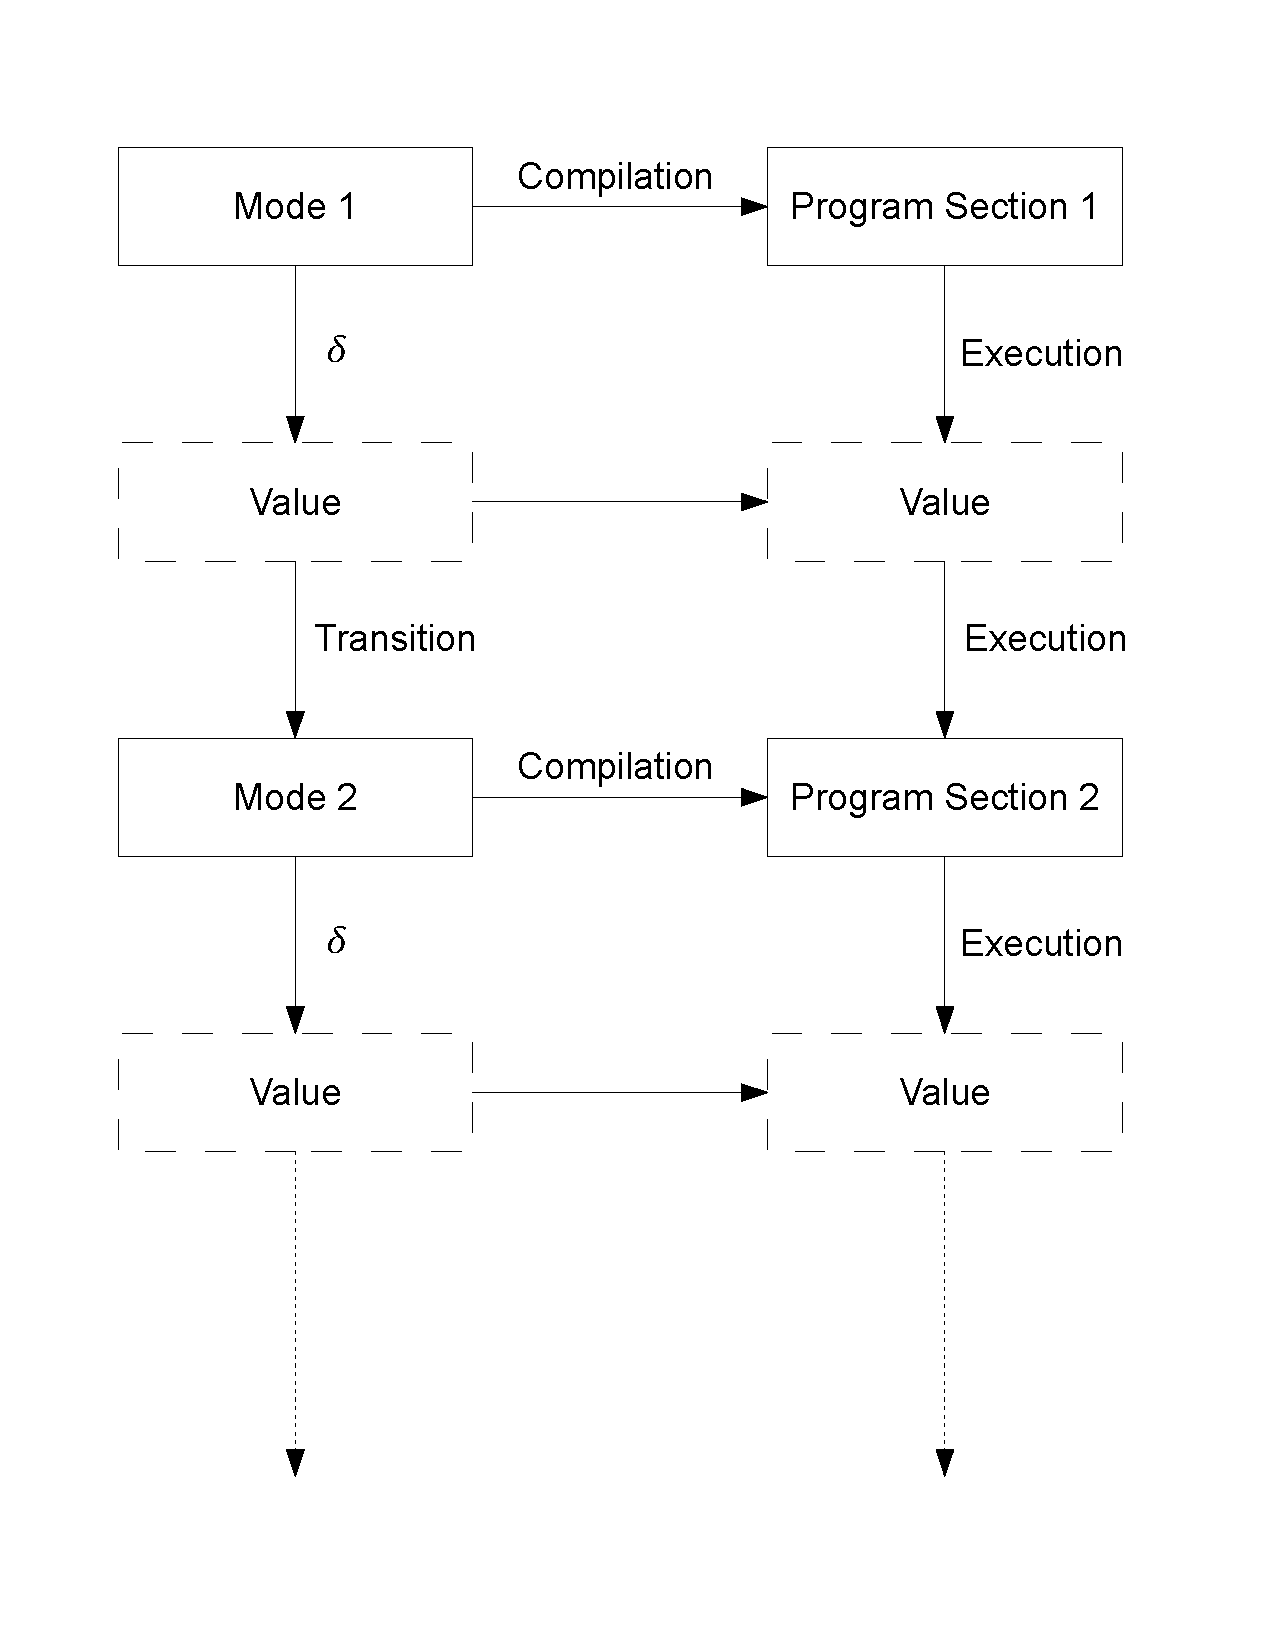
\includegraphics[trim= 10mm 30mm 10mm 10mm, clip, width=\imgmedium]{./images/correctness_graph2.pdf}
    \caption{Code Transition Structure}
    \label{fig:correctness_graph2}
\end{figure}
generated from an graph structure is correct. To do so we extend figure \ref{fig:correctness_graph1} iteratively to obtain figure \ref{fig:correctness_graph2} to evaluate the transitions.

In this section we will begin by showing that each of the transformations are correct by constructing basic atoms. We will start by looking at atoms that have the simpliest expressions first. The simplest of these is a diagram in which only the start node exists as shown in \ref{fig:correctness_ex_start}.

\begin{figure}[htb]
	\centering
	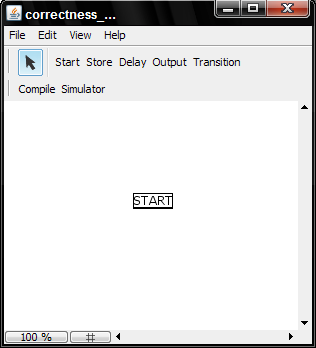
\includegraphics[width=\imgmedphoto]{./images/correctness_ex_start.png}
	\caption{Singular Start Block}
	\label{fig:correctness_ex_start}
\end{figure}
In this simple example the following generated intermediate code \emphasize{IL} is created.

\noindent\begin{minipage}{\textwidth}
\begin{lstlisting}[frame=single]
// VARIABLE DECLARATIONS //
BLUID0:
//////////////////////////////////////
//        PROGRAM START             //
//////////////////////////////////////
goto EOF;

EOF:
return;
\end{lstlisting}
\end{minipage}

In this simplest example we have a label inserted at the beginning of the start block so we can re-enter the start block namely BLUID0. Following the label a comment header to denote the block type, and no variables declared.  Because there is no other transition or block an automatic transition to \emphasize{EOF} is setup in order to terminate the program.

\begin{figure}[htb]
	\centering
	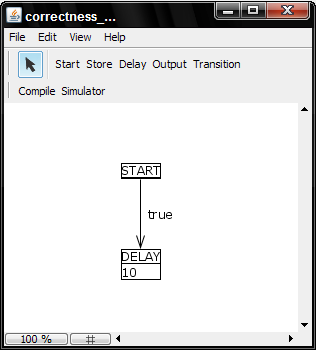
\includegraphics[width=\imgmedphoto]{./images/correctness_ex_delay.png}
	\caption{Delay Block Block}
	\label{fig:correctness_ex_delay}
\end{figure}

Moving up in complexity we have a start block followed by our next simpliest element the delay block, joined by one transition leaving the start block. We can see from figure \ref{fig:correctness_ex_delay}
the structure of this new graph. We will use this example to examine transitions are compiled into final code, but first we shall look at the delay block itself.

\noindent\begin{minipage}{\textwidth}
\begin{lstlisting}[frame=single]
// VARIABLE DECLARATIONS //
...

BLUID1:
//////////////////////////////////////
//        DELAY                     //
//////////////////////////////////////
delayms(10);
goto EOF;

EOF:
return;
\end{lstlisting}
\end{minipage}

The delay block itself has a structure identical to the start block. The only difference in this case is the delay block doesn't have a null code section. The delay block generates one line of code, namely delay(integer). The actual delay routine is implimented on the driver level per device since certain devices lack internal timers. It will be up to each implementor to ensure that the delay will correctly delay each the integer specified (in milliseconds). 

\noindent\begin{minipage}{\textwidth}
\begin{lstlisting}[frame=single]
// VARIABLE DECLARATIONS //
BLUID0:
//////////////////////////////////////
//        PROGRAM START             //
//////////////////////////////////////
goto BLUID1;
goto EOF;

BLUID1:
//////////////////////////////////////
//        DELAY                     //
//////////////////////////////////////
delayms(10);
goto EOF;

EOF:
return;
\end{lstlisting}
\end{minipage}

In this basic example transitions are actually used at this point. The reader will observe that we have directly mapped each edge to a goto statement that is guarded by the guard condition on the edge itself. As defined in section \ref{sec:statechartsyn} the transitions are always mutually exclusive and to not do so would be considered a syntax error. The reason is there is no way to enforce sequence in which each edge is evaluated that would make sense to the programmer constructing the diagram in a visual way. It is up to the programmer (diagram constructor) to ensure that we never run into a condition where two edges actually have an area of overlap.

Each block has an unique identitifer associated with it, this identifier is what is used by the goto blocks in order to recreate the graph structure in the code. The unique identifier is generated at design time and is checked at compile time to ensure that it is in fact unique.


%the lower sections might be superceeded by the above.
\subsection{The IL}
\subsection{The Generated Code Sections}
\subsection{The Simulator}